\cleardoublepage\chapter{Specifications}\minitoc\vspace{.5cm}

\section{Specification 1}\index{Specification 1}

\todomid{write about \Cref{lst:spec1}}

\lstset{language=ttl, breaklines=true, caption=Specification 1, %
emptylines=0,
label=lst:spec1, numbers=left, stepnumber=1, inputencoding=utf8}
\lstinputlisting{resources/code/example.java}


\section{Specification 2}\index{Specification 2}

\todomid{write about \Cref{lst:spec2}}

\lstset{language=ttl, breaklines=true, caption=Specification 2, %
emptylines=0,
label=lst:spec2, numbers=left, stepnumber=1, inputencoding=utf8}
\lstinputlisting{resources/code/example.java}


\cleardoublepage\chapter{Test Results}\minitoc\vspace{.5cm}

\section{Conformance Results}

\sidenote{Overview}
\todomid{write about \Cref{fig:test:result1,fig:test:result2}}

\begin{figure}[H]
    \centering
    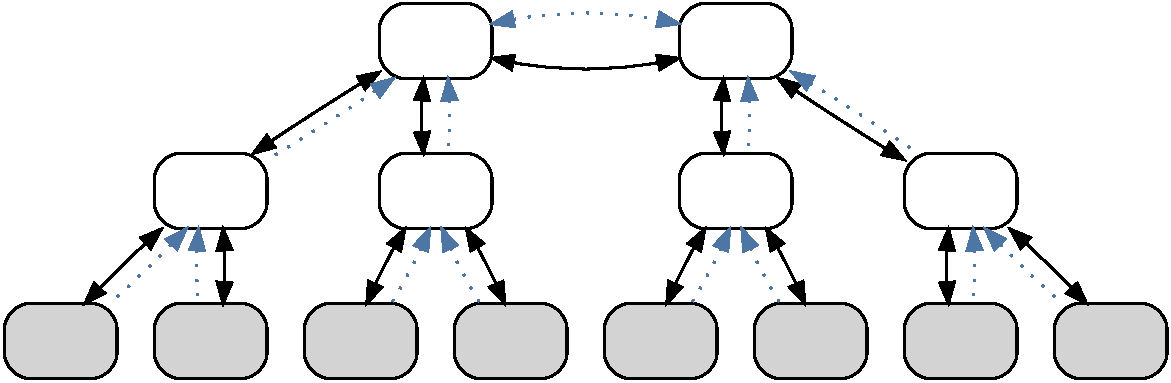
\includegraphics[width=.9\textwidth,frame,page=1]{resources/images/example3}
    \caption{Test results (page 1)}\label{fig:test:result1}
\end{figure}

\begin{figure}[H]
    \centering
    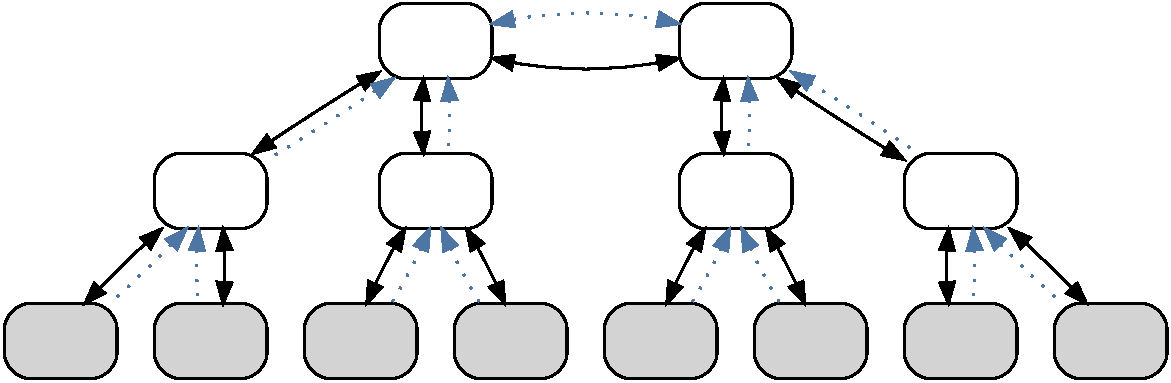
\includegraphics[width=.9\textwidth,frame,page=1]{resources/images/example3}
    \caption{Test results (page 2)}\label{fig:test:result2}
\end{figure}

\section{Performance Results}

\subsection{Histograms}

\sidenote{Overview}
\todomid{write about \Cref{fig:eval:perf:hist:forms}}

\begin{figure}[H]
    \begin{subfigure}[b]{.5\textwidth}
      \centering
      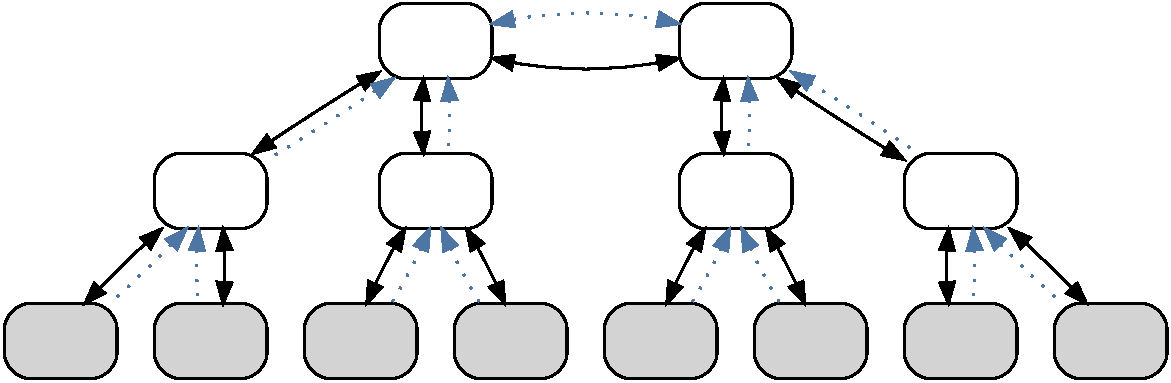
\includegraphics[width=.95\textwidth,frame]{resources/images/example3}
      \caption{Form A}
    \end{subfigure}~\begin{subfigure}[b]{.5\textwidth}
      \centering
      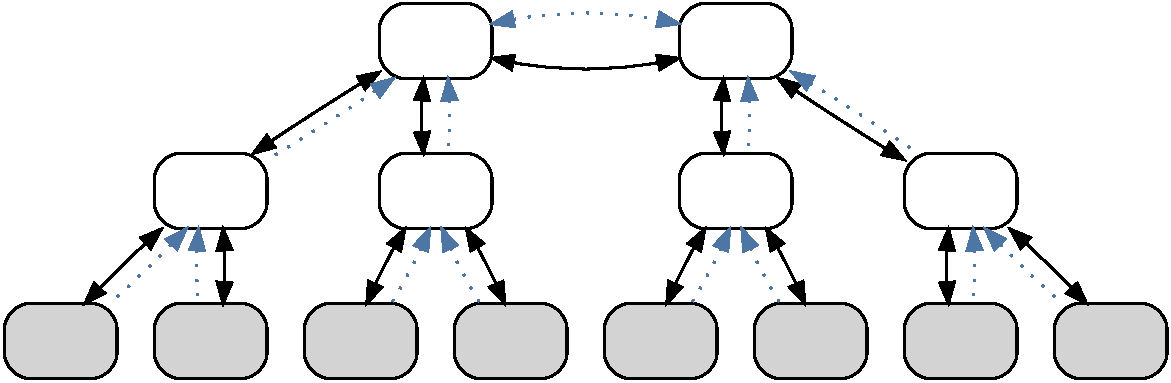
\includegraphics[width=.95\textwidth,frame]{resources/images/example3}
      \caption{Form B}
    \end{subfigure}
    \caption{Histogram of Forms}\label{fig:eval:perf:hist:forms}
\end{figure}


\subsection{Lineplots}

\sidenote{Overview}
\todomid{write about \Cref{fig:eval:perf:line:lines}}

\begin{figure}[H]
    \begin{subfigure}[b]{.5\textwidth}
      \centering
      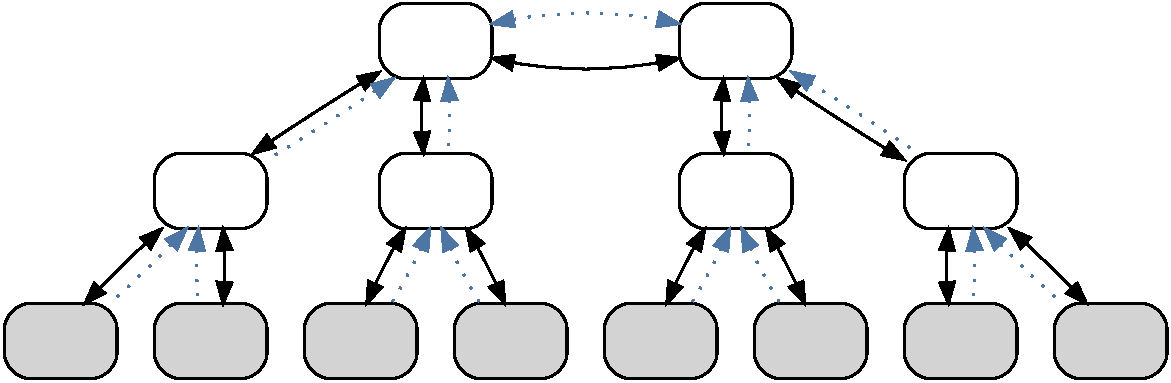
\includegraphics[width=.95\textwidth,frame]{resources/images/example3}
      \caption{Lines A}
    \end{subfigure}~\begin{subfigure}[b]{.5\textwidth}
      \centering
      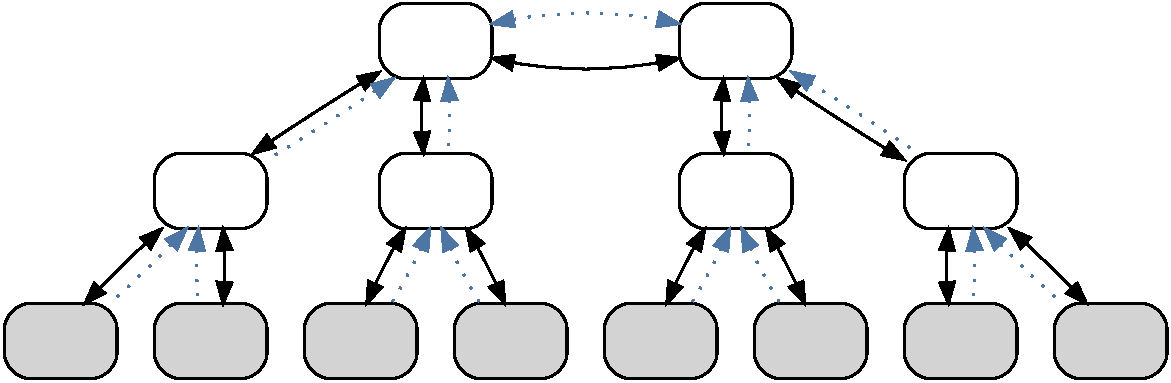
\includegraphics[width=.95\textwidth,frame]{resources/images/example3}
      \caption{Lines A}
    \end{subfigure}
    \caption{Lineplot of the lines}\label{fig:eval:perf:line:lines}
\end{figure}
